\chapter{Implementation}
The Links compiler is a multi-pass compiler with several distinct phases.
Coarsely, we can divide the compiler into two major components the front-end and back-end.
We can further subdivide the front-end into
\begin{itemize}
  \item Parser: Transforms the input source into a syntax tree.
  \item Early desugar: Performs source-to-source transformations before source analysis.
  \item Type checker: Analyses the source, performs type inference, and ensures terms are well-typed.
\end{itemize}
The compiler has more front-end components, but these are the most relevant for our implementation.
Similarly, the back-end can be further subdivided
\begin{itemize}
  \item IR Compiler: Transforms the source into an intermediate representation used by the interpreter.
  \item Pattern-matching compiler: Aids the IR compiler by compiling pattern-matching constructs into the intermediate representation.
\end{itemize}
Figure \ref{fig:compiler-phases} provides a high level picture of how the different relevant phases are connected. The subsequent sections discuss implementation specific details.
\begin{figure}[t]
\begin{center}
\tikzset{my ellipse/.style={
        draw=blue, 
        ultra thick, 
        rectangle, 
        anchor=west, 
        xshift=1.0cm},
}
\tikzset{my rectangle/.style={
        draw=black, 
        thick, 
        rectangle, 
        minimum width={width("Early desugar")+2pt}}
}
\tikzset{my arrow/.style={-latex, thick}}

\begin{tikzpicture}  
  % Frontend
  \node [my rectangle,draw=black,thick] (Early desugar) at (0,0) {Early desugar};
  \node [my rectangle,draw=black,thick,above of=Early desugar] (Parser) {Parser};
  \node [my rectangle,draw=black,thick,below of=Early desugar] (Typechecker) {Type checker};
  %\node [my rectangle,draw=black,thick,below of=Typechecker] (Late desugar) {Late desugar};

  \node[rectangle,draw=black,ultra thick,minimum height=+5.0cm,minimum width=+4.0cm,fit ={(Parser.north) (Typechecker.south)}] (Frontend) {};

  % Input source
  \node [rectangle,draw=black,thick,xshift=-3.0cm,left of=Frontend] (Source) {Source};

  % Backend
  \node [my rectangle,xshift=+4.0cm,draw=black,thick,right of=Parser] (Sugartoir) {IR Compiler};
  \node [my rectangle,yshift=-0.5cm,draw=black,thick,below of=Sugartoir] (PMC) {\begin{tabular}{l}Pattern\\Matching\\ Compiler\end{tabular}};
  
  \node[rectangle,draw=black,ultra thick,minimum width=+4.0cm,minimum height=+5.0cm,fit ={(Sugartoir.north) (PMC.south)}] (Backend) {};

  % Interpreter
  \node [rectangle,xshift=+3.5cm,draw=black,thick,right of=Backend] (Evalir) {Interpreter};

  % Texts
  \node [anchor=north, font=\bfseries,yshift=-0.1cm] at (Frontend.north) {Frontend};
  \node [anchor=north, font=\bfseries,yshift=-0.1cm] at (Backend.north) {Backend};

  % Arrows
  \draw [->, ultra thick] (Source.east) -- (Frontend.west) {};
  \draw [->, ultra thick] (Frontend.east) -- (Backend.west) {};
  \draw [->, ultra thick] (Backend.east) -- (Evalir.west) {};

  \draw [->, thick] (Parser.south) -- (Early desugar.north) {};
  \draw [->, thick] (Early desugar.south) -- (Typechecker.north) {};

  \draw [->, thick,out=150, in=20] (Sugartoir.-10.-150) -- (PMC.135.0) {};
  \draw [->, thick] (PMC.43.0) -- (Sugartoir.-19.0) {};
\end{tikzpicture}
\caption{Links compiler phases overview.}\label{fig:compiler-phases}
\end{center}
\end{figure}

\section{Early desugaring of handlers}
The \code{handler} and \code{open handler} constructs are syntactic sugar. They get desugared into a legacy construct from an early implementation. The initial implementation used a \code{handle}-construct for handlers. Figure \ref{fig:closedhandler-desugar} displays the conceptual transformation of \code{handler} to \code{handle}. 
This desugaring takes place right after the parsing phase. The early desugaring is beneficial because it allows us to take full advantage of the earlier implementation, whilst providing a more convenient syntax for handlers.
\begin{figure}[h]
    \centering
    \begin{subfigure}[c]{0.45\textwidth}
        \centering
\begin{lstlisting}[style=links]
handler(m) {
  case Op§*$_i$*§(p§*$_i$*§,k§*$_i$*§) -> b§*$_i$*§
  case Return(x) -> b
}
\end{lstlisting}
    \end{subfigure}%
    ~ 
    \begin{subfigure}[c]{0.1\textwidth}
      $\Rightarrow$
    \end{subfigure}%
    ~
    \begin{subfigure}[c]{0.45\textwidth}
        \centering
\begin{lstlisting}[style=links]
fun(m) {
  handle(m) {
    case Op§*$_i$*§(p§*$_i$*§,k§*$_i$*§) -> b§*$_i$*§
    case Return(x) -> b
  }
}
\end{lstlisting}
    \end{subfigure}
\caption{The \code{handler}-construct gets desugared into a \code{handle}-construct where the computation $m$ is abstracted over using a function.}\label{fig:closedhandler-desugar}
\end{figure}

The \code{open handler}-constructs get desugared in a similar fashion, but, with a small twist: The \code{handle}-construct gets wrapped inside a thunk. The extra layer of indirection entailed by this transformation is \emph{the key} to make handlers composable. The crucial insight is that by transforming every open handler into a thunk compositionality follows for free because computations are modelled as thunks.
Figure \ref{fig:openhandler-desugar} shows the conceptual transformation for \code{open handler}-constructs.

\begin{figure}[h]
    \centering
    \begin{subfigure}[c]{0.45\textwidth}
        \centering
\begin{lstlisting}[style=links]
open handler(m) {
  case Op§*$_i$*§(p§*$_i$*§,k§*$_i$*§) -> b§*$_i$*§
  case Return(x) -> b
}
\end{lstlisting}        
    \end{subfigure}%
    ~ 
    \begin{subfigure}[c]{0.1\textwidth}
      $\Rightarrow$
    \end{subfigure}%
    ~
    \begin{subfigure}[c]{0.45\textwidth}
        \centering
\begin{lstlisting}[style=links]
fun(m) {
  fun() {
    handle(m) {
      case Op§*$_i$*§(p§*$_i$*§,k§*$_i$*§) -> b§*$_i$*§
      case Return(x) -> b
    }
  }
}
\end{lstlisting}       
    \end{subfigure}
\caption{The \code{open handler}-construct gets desugared into a thunked \code{handle}-construct.}\label{fig:openhandler-desugar}
\end{figure}

\section{Type inference}
\[
\mprset{flushleft}
\inferrule{E_{in} \defas \{\type{Op}_i : a_i \to b_i\}_i \uplus \rho \\\\
           E_{out} \defas E_{\alpha} \uplus \rho\\\\
           H \defas \{\code{Return}(x) \mapsto M\} \uplus \{\type{Op}_i(p,k) \mapsto N_i\}_i \\\\
          \left( \varGamma, p : a_i, k : U_{E_{out}}(b_i \to c) \vdash_{E_{out}} N_i : c \right)_i \\\\
          \varGamma, x : A \vdash_{E_{out}} M : C}
          {\varGamma \vdash H : a\, \overset{E_{in}\;\;\;E_{out}}{\Rightarrow} c}
\]
\section{Pattern-matching compilation}
Syntactically, the \code{handler}-construct and \code{switch}-construct are similar. Figure \ref{fig:handler-switch} puts the two construct side-by-side.
\begin{figure}[h]
    \centering
    \begin{subfigure}[c]{0.45\textwidth}
        \centering
\begin{lstlisting}[style=links]
handler(m) {
  case Op§*$_i$*§(p§*$_i$*§,k§*$_i$*§) -> b§*$_i$*§
  case Return(x) -> b
}
\end{lstlisting}        
    \end{subfigure}%  
    ~
    \begin{subfigure}[c]{0.45\textwidth}
        \centering
\begin{lstlisting}[style=links]
switch(e) {
  case §*$\textit{Pattern}_j$*§ -> b§*$_j$*§
  case other   -> b§*$'$*§
}
\end{lstlisting}       
    \end{subfigure}
\caption{The \code{handler}-construct resembles the \code{switch}-construct syntactically.}\label{fig:handler-switch}
\end{figure}
Notably, their semantics differ as \code{switch} allows arbitrary pattern matching on an expression $x$ and \code{handler} only allows pattern matching on possible operation names in some computation $m$. Furthermore, \code{switch} has a default case \code{other} which is not allowed in \code{handler}. 
Their syntactic similarities give rise to a similar internal representation as well. Although, the internal representation of \code{handler} contains extra attributes such as whether the handler is open or closed.
The resemblance has certain benefits:
\begin{itemize}
  \item Syntactical commonalities makes handlers feel like a natural integrated part in Links,
  \item and we can reuse the \code{switch} pattern-matching compilation infrastructure for \code{handler}.
\end{itemize}
The \code{switch} pattern-matching compiler supports deep pattern-matching which we want for matching on actual operation parameters, but only a handful of patterns are permitted for matching on continuation parameters. Figure \ref{fig:cont-pattern-matching} shows the legal pattern-matching for the continuation parameter. Moreover, the \code{Return}-case must only take one parameter. These small subtleties prevent us from using the \code{switch} pattern-matching compiler directly.

\begin{figure}[H]
\begin{center}
\begin{lstlisting}[style=links]
         handler(m) {
           case Op§*$_{i_1}$*§(_,k)      -> b§*$_{i_1}$*§  # Name binding
           case Op§*$_{i_2}$*§(_,k as c) -> b§*$_{i_2}$*§  # Aliasing
           case Op§*$_{i_3}$*§(_,_)      -> b§*$_{i_3}$*§  # Wildcarding
           case Return(x)     -> b§*$_{i_4}$*§
         }
\end{lstlisting}        
\end{center}
\caption{Permissible patterns for matching on the continuation parameter.}\label{fig:cont-pattern-matching}
\end{figure}

Instead we embed the \code{switch} pattern-matching compiler along with a preliminary pattern-matching analyser in the \code{handler} pattern-matching compiler. The pattern-matching analyser checks that the patterns are legal, i.e.
\begin{itemize}
  \item An operation-case has at least two parameters, where the last parameter is supposed to be the continuation.
  \item Pattern-matching on a continuation parameter is either name binding, aliasing or wildcarding.
  \item \code{Return}-case(s) only take one parameter.
\end{itemize}
If the pattern-matching analysis is successful then the \code{switch} pattern matching compiler is invoked to generate the code. Otherwise, a compilation error, complaining about illegal patterns, is emitted.

\section{Interpreter}
% Continuation passing style (CPS) is often used as an intermediate representation during the optimisation stage by functional compilers. In particular, CPS makes it easy to implement first-class control in the source level as CPS exposes the current continuation \cite{Appel2007}.

% A related intermediate representation is A-Normal Form (ANF) which is used by the Links compiler. Furthermore, the Links interpreter directly interprets ANF code \cite{Lindley2012}.
% ANF is a relatively simple language that enjoys many of the same advantages as CPS such as explicit exposure of the current continuation \cite{Flanagan1993}. However, CPS is better for performing optimisations, but the simpler nature of ANF makes it amendable as an interpreted language \cite{Appel2007,Flanagan1993}. 
The Links compiler uses A-Normal Form (ANF) as an intermediate representation. In particular, the Links interpreter directly interprets ANF code.
ANF is a relatively simple direct-style language which partitions expressions into two classes: atomic expressions and complex expressions. An expression is considered atomic if it is pure, i.e. it causes no effects and it terminates \cite{Flanagan1993}. On the other hand, every complex expression must be assigned a fresh name. For example the Links expression \code{g(f(h(x)))} gets translated into the Links-ANF computation \code{($\{$let y = h(x), let z = f(y)$\}$, g(z))} where the first component is a list of \code{let}-bound intermediate computations, and the second component is a tail computation. Incidentally, it is straightforward to implement first-class control in the source language as the current continuation can be built from the Links-ANF computation. Moreover, the simplicity of ANF makes it amendable as an interpreted language.

The Links interpreter is written in continuation-passing style (CPS) which threads the current continuation directly through the program. The continuation was implemented as a stack of continuation frames which capture computations along with their contexts. Formally, a continuation frame is quadruple $F \defas (\mathcal{S},\mathcal{B},\mathcal{E},\mathcal{C})$ where
\begin{itemize}
  \item $\mathcal{C}$ is a computation.
  \item $\mathcal{E}$ is an environment that binds names in $\mathcal{C}$.
  \item $\mathcal{B}$ is a binder for the computation.
  \item $\mathcal{S}$ denotes the scope of the computation.
\end{itemize}
For example the expression above gets encoded as the following continuation frame
\[ \left( \text{scope}(\code{y}), \code{y}, \text{localise}(\code{y}), \code{(\{let z = f(y)\}, g(z))} \right) \]
where scope and localise are two functions, that return the scope of a binder and localises the binder in the current environment, respectively.

This particular notion of continuation is problematic for handlers because we need delimited control for continuations assigned by handlers. Therefore it is necessary to generalise the notion of continuation in the Links interpreter. Fortunately, the generalisation is conceptual simple: Lift the continuation into a stack, i.e. let it become a stack of stacks of continuation frames. In other words the generalised continuation embeds the previous continuation layout. Figure \ref{fig:continuation-notion} illustrates the embedding. This scheme effectively turns every stack of continuation frames into a delimited continuation, i.e. a continuation that returns control to the caller.

\begin{figure}[H]
\begin{center}
\tikzset{my ellipse/.style={
        draw=blue, 
        ultra thick, 
        rectangle, 
        anchor=west, 
        xshift=1.0cm},
}
\tikzset{my rectangle/.style={
        draw=black, 
        thick, 
        rectangle, 
        minimum width={width("Early desugar")+2pt}}
}

\tikzset{my arrow/.style={-latex, thick}}

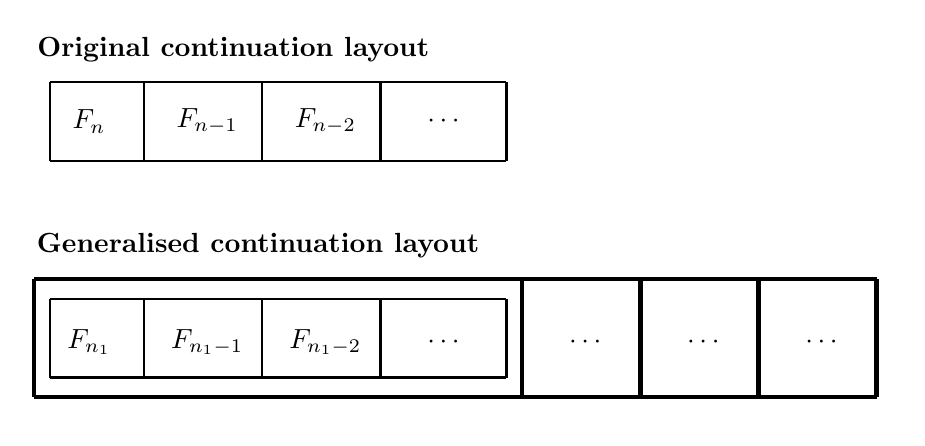
\begin{tikzpicture}  
  % Previous continuation
  % Draw rectangle
  \draw[thick,-] (-2.8,0) -- (-2.8,1.0) node[xshift=0.5cm] {};   % Left bar
  \draw[thick,-] (-2.8,1.0) -- (3.0,1.0) node[anchor=north west] (top) {}; % top
  \draw[thick,-] (-2.8,0) -- (3.0,0) node[anchor=north west] {};     % bottom
  \draw[thick,-] (3.0,0) -- (3.0,1.0) node[anchor=north west] {}; % Right bar

  % Draw cell separators
  \foreach \x in {-1.6,-0.1,1.4}
     \draw[thick,-] (\x,0) -- (\x,1.0) {};

  % Draw cell contents
  \draw (-2.3 cm,0) -- (-2.3 cm,0) node[yshift=0.5cm] {$F_{n}$};
  \draw (-0.8 cm,0) -- (-0.8 cm,0) node[yshift=0.5cm] {$F_{n-1}$};
  \draw (0.7 cm,0) -- (0.7 cm,0) node[yshift=0.5cm] {$F_{n-2}$};
  \draw (2.2 cm,0) -- (2.2 cm,0) node[yshift=0.5cm] {$\cdots$};

  % Generalised continuation
  \draw[ultra thick,-] (-3,-3.0) -- (-3,-1.5) node[xshift=0.5cm] {};   % Left bar
  \draw[ultra thick,-] (-3,-1.5) -- (7.7,-1.5) node[anchor=north west] (gtop) {}; % top
  \draw[ultra thick,-] (-3,-3.0) -- (7.7,-3.0) node[anchor=north west] {};     % bottom
  \draw[ultra thick,-] (7.7,-3.0) -- (7.7,-1.5) node[anchor=north west] {}; % Right bar


  % Draw inner continuation rectangle
  % Draw rectangle
  \draw[thick,-] (-2.8,-2.75) -- (-2.8,-1.75) node[xshift=0.5cm] {};   % Left bar
  \draw[thick,-] (-2.8,-1.75) -- (3.0,-1.75) node[anchor=north west] {}; % top
  \draw[thick,-] (-2.8,-2.75) -- (3.0,-2.75) node[anchor=north west] {};     % bottom
  \draw[thick,-] (3.0,-2.75) -- (3.0,-1.75) node[anchor=north west] {}; % Right bar

  % Draw first inner continuation cell contents
  \draw (-2.3 cm,-3.0) -- (-2.3 cm,-3.0) node[yshift=0.7cm] {$F_{n_1}$};
  \draw (-0.8 cm,-3.0) -- (-0.8 cm,-3.0) node[yshift=0.7cm] {$F_{n_1-1}$};
  \draw (0.7 cm,-3.0) -- (0.7 cm,-3.0) node[yshift=0.7cm] {$F_{n_1-2}$};
  \draw (2.2 cm,-3.0) -- (2.2 cm,-3.0) node[yshift=0.7cm] {$\cdots$};

  % Draw inner continuation cell separators
  \foreach \x in {-1.6,-0.1,1.4}
     \draw[thick,-] (\x,-2.75) -- (\x,-1.75) {};

  % Draw continuation separators
  \draw[ultra thick,-] (3.2cm, -3.0) -- (3.2cm, -1.5) node {};
  \draw[ultra thick,-] (4.7cm, -3.0) -- (4.7cm, -1.5) node {};
  \draw[ultra thick,-] (6.2cm, -3.0) -- (6.2cm, -1.5) node {};
  \draw (3.5cm, -3.0) -- (4.0 cm, -3.0) node[draw=none,yshift=0.7cm] {$\cdots$};
  \draw (5.2cm, -3.0) -- (5.5 cm, -3.0) node[draw=none,yshift=0.7cm] {$\cdots$};
  \draw (6.5cm, -3.0) -- (7.0 cm, -3.0) node[draw=none,yshift=0.7cm] {$\cdots$};

  % Texts
  \node [anchor=north, font=\bfseries,yshift=0.7cm,xshift=-8.0cm] at (gtop.north) {Generalised continuation layout};
  \node [anchor=north, font=\bfseries,yshift=0.7cm,xshift=-3.6cm] at (top.north) {Original continuation layout};
\end{tikzpicture}
\caption{The generalised continuation embeds the previous continuation layout.}\label{fig:continuation-notion}
\end{center}
\end{figure}

The generalised continuation is built in parallel with a stack of handlers. Whenever the interpreter encounters a handler, it pushes the handler onto the handlers' stack and allocates a new delimited continuation which is pushed onto the stack inside the generalised continuation. The top-most delimited continuation grows as the evaluation progresses. Conversely, when the top-most delimited continuation is depleted the proper \code{Return}-case of the top-most handler is invoked. Additionally, both elements are popped from their respective stacks. The evaluation terminates when the entire generalised continuation has been consumed.

Operation invocation follows a rather simple scheme: Upon encountering an operation the interpreter pops and invokes the top-most handler, if the handler does not handle the operation, then the second top-most handler is popped and invoked and so forth. The interpreter maintains the popped handlers in a separate temporary stack along with their corresponding delimited continuations. The temporary stack is a ``slice'' of the program state which is assigned to the continuation parameter when a matching case is found. If no matching case is found then an ``unhandled operation'' error is emitted. When the continuation is invoked the ``sliced'' state is merged back into the program state. This ensures that the \code{Return}-cases are invoked in the proper order when the handled computation finishes.
